\documentclass{article}

\usepackage[
margin=0in,
paperwidth=12.723in,  % 6.125 + 0.473 + 6.125  (WEISS, 210 Seiten)
paperheight=9.25in
]{geometry}

\usepackage{graphicx}
\usepackage{tikz}
\usetikzlibrary{calc}
\usepackage{xcolor}
\pagestyle{empty}

% Maße
\newlength{\panel}
\setlength{\panel}{6.125in}     % Rückseite/Vorderseite inkl. Bleed

\newlength{\spine}
\setlength{\spine}{0.473in}     % Rückenbreite

\newlength{\coverheight}
\setlength{\coverheight}{9.25in}

% Farben
\definecolor{coverblue}{HTML}{1E4A66}
\definecolor{spinebg}{HTML}{E6D8B9} % warmes Beige

\begin{document}
	
	\begin{tikzpicture}[remember picture,overlay]
		
		% Seitenreferenz
		\coordinate (SW) at (current page.south west);
		
		% -------------------------------------------------
		% Rückseite links
		% -------------------------------------------------
		\node[anchor=south west, inner sep=0pt] 
		at (SW)
		{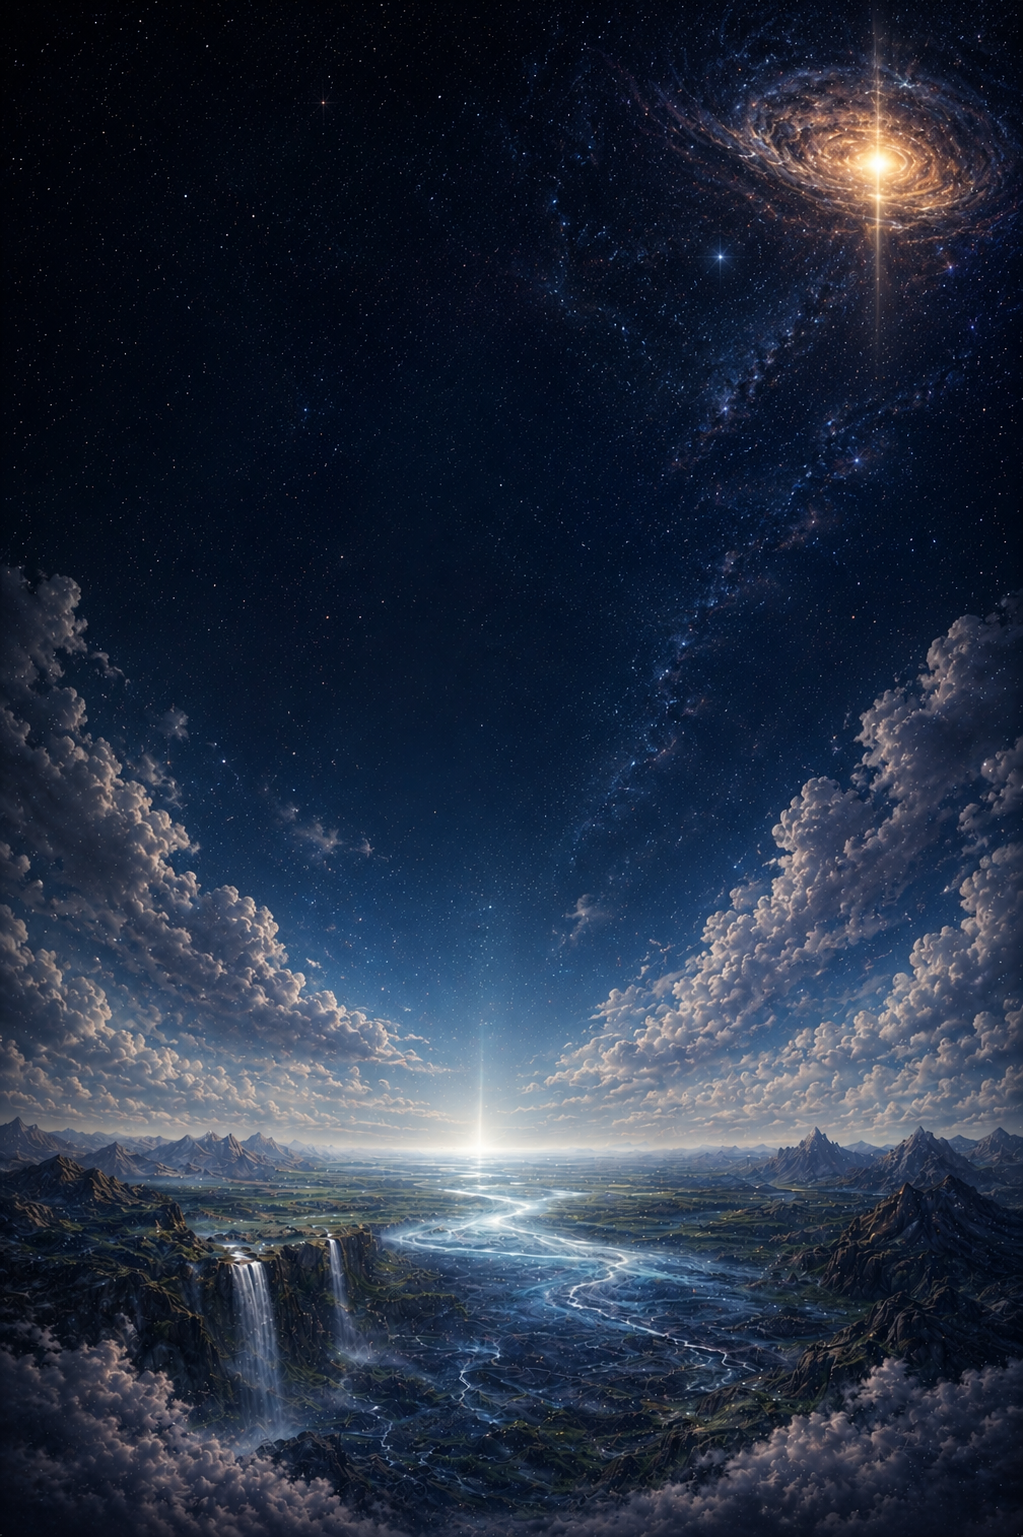
\includegraphics[
			width=\panel,
			height=\coverheight,
			pagebox=mediabox
			]{rueckseite.pdf}};
		
		% -------------------------------------------------
		% Rücken exakt zwischen Rückseite und Vorderseite
		% -------------------------------------------------
		\fill[spinebg] 
		($(SW)+(\panel,0)$) 
		rectangle 
		++(\spine,\coverheight);
		
		% -------------------------------------------------
		% Vorderseite rechts
		% -------------------------------------------------
		\node[anchor=south west, inner sep=0pt] 
		at ($(SW)+(\panel+\spine,0)$)
		{\includegraphics[
			width=\panel,
			height=\coverheight,
			pagebox=mediabox
			]{vorderseite.pdf}};
		
		% -------------------------------------------------
		% Rücken-Text exakt auf Rückenmitte
		% -------------------------------------------------
		\node[rotate=90, align=center, text=coverblue]
		at ($(SW)+(\panel+0.5*\spine,0.5*\coverheight)$)
		{
			\bfseries\large
			Christian Weilharter
			\hspace*{1.5cm}
			Die Struktur der Welt
		};
		
		% -------------------------------------------------
		% Kontrolllinien: später auskommentieren
		% -------------------------------------------------
		%\draw[red, line width=0.3pt] 
	%	($(SW)+(\panel,0)$) -- ($(SW)+(\panel,\coverheight)$);
		
		%\draw[red, line width=0.3pt] 
	%	($(SW)+(\panel+\spine,0)$) -- ($(SW)+(\panel+\spine,\coverheight)$);
		
	%	\draw[blue, line width=0.3pt] 
	%	($(SW)+(\panel+0.5*\spine,0)$) -- ($(SW)+(\panel+0.5*\spine,\coverheight)$);
		
	\end{tikzpicture}
	
\end{document}